\documentclass[a4paper,10pt]{article}
\usepackage{tikz}
\usepackage{geometry}
\usepackage{float}
\usetikzlibrary{shapes,positioning,calc,arrows.meta}
\colorlet{lightgray}{gray!30}
\usepackage{xcolor}
\usepackage{amsmath}
\usepackage[pdfusetitle,linkcolor=black,pdfborder={0,0,0}]{hyperref}

\geometry{a4paper,top=1.0in,bottom=1.0in,left=1.0in,right=1.0in}

\author{ \Large \textbf{\emph{Akash Kishore}}}

\date{\Large April 2020}

\title{\Huge \textbf{Learning Tikz}}

\begin{document}
\maketitle

\large
%Hello, this is $\int^1_2\int^3_4 f(x,y)dxdy$
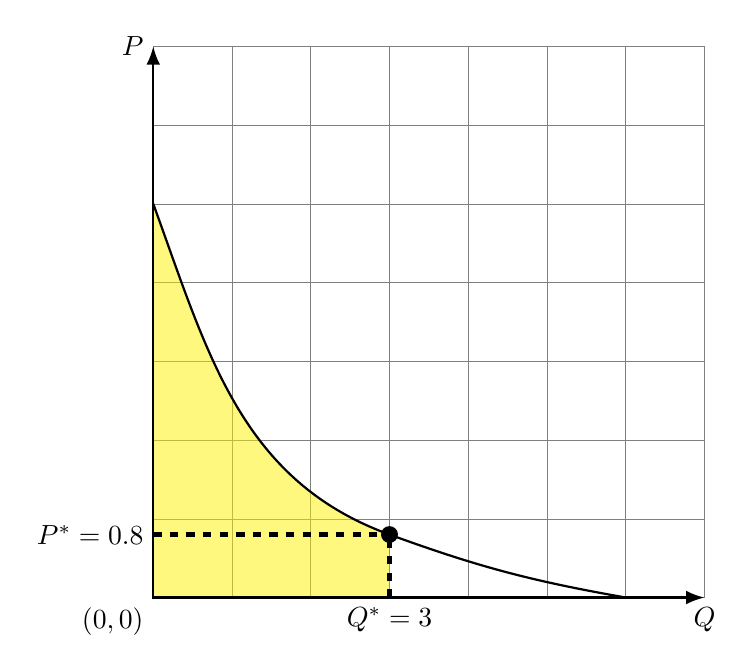
\begin{tikzpicture}[>={Latex}]
	\draw[help lines] (0,0) grid (7,7);
	\draw (0,7) node [left] {$P$};
	\draw (0,0) node [below left] {$(0,0)$};
	\draw (7,0) node [below] {$Q$};
	\path[fill=yellow,fill opacity=0.5] (0,0) -- (0,5) to [out=-70,in=160] (3,.8) -- (3,0) -- (0,0);
	\draw[thick] (0,5) to [out=-70,in=160] (3,.8) to [out=-20, in=170] (6,0);
	\draw[fill] (3,0.8) circle [radius=0.1];
	\draw[dashed,ultra thick] (0,.8) -- (3,.8);
	\draw[dashed,ultra thick] (3,0) -- (3,.8);
	\draw[<->,thick] (0,7) |- (7,0);
	\draw (0,.8) node [left] {$P^* = 0.8$};
	\draw (3,0) node [below] {$Q^* = 3$};
	
\end{tikzpicture}
\end{document}
